% ===== neural-networks =====
\section*{Neural Networks}
% ---- CS189 scope checklist: must include ([x] = already covered) ----
% Source: Lecture 12; reference sheet p.8
% [ ] Linear models fail on XOR (fixed basis functions)
% [ ] Neuron = weighted sum + activation; perceptron (step activation)   (weighted sum + sigmoid done; perceptron not yet)
% [ ] XOR with two layers: hidden units are learned features
% [x] Fully connected layer z = W h + b, h = phi(z); parameter count D_out(D_in + 1)
% [ ] Without nonlinear activations, stacked layers collapse into one linear model
% [ ] Activations and derivatives: sigmoid (max slope 1/4), tanh, ReLU   (sigmoid shape only)
% [ ] Output layer + loss: identity + MSE, sigmoid + cross-entropy, softmax + cross-entropy
% ----

\subsection*{Why Neural Networks?}
Its easy for your brain to recognize a low-resolution 3 as a 3 without effort, even though no two 3's have the same pixels. But try writing a program that takes in a $28 \times 28$ grid of pixels and outputs the digit, and it suddenly becomes very hard. A neural network gets around this by learning from examples.

\subsection*{Running Example: Reading Handwritten Digits}
\begin{keeptogether}
Input: a $28 \times 28$ grayscale image $\mathbf{x}$. Output: which of $K = 10$ classes (digits 0--9) it is.
\begin{itemize}
  \item A \textbf{neuron} (or \textbf{unit}) holds one number, its \textbf{activation} $h$. Here it's between 0 and 1.
  \item \textbf{Input layer:} one unit per pixel, so $\mathbf{x} \in \mathbb{R}^{D}$ with $D = 28 \times 28 = 784$. Each $x_d$ is pixel $d$'s brightness: 0 = black, 1 = white.
  \item \textbf{Output layer:} $K = 10$ units, one per class. Unit $k$'s activation $\hat{y}_k$ is how strongly the network thinks the image is digit $k$. The prediction is the $k$ with the largest $\hat{y}_k$.
  \item \textbf{Hidden layers:} two layers of 16 units in between, $\mathbf{h}^{(1)}$ and $\mathbf{h}^{(2)}$ (16 is an arbitrary choice).
  \item \textbf{Fully connected, feed-forward:} every unit gets input from every unit in the layer before it, so each layer's activations are computed from the previous layer's. Computing $\mathbf{x} \to \mathbf{h}^{(1)} \to \mathbf{h}^{(2)} \to \hat{\mathbf{y}}$ is the \textbf{forward pass}.
\end{itemize}

{\centering
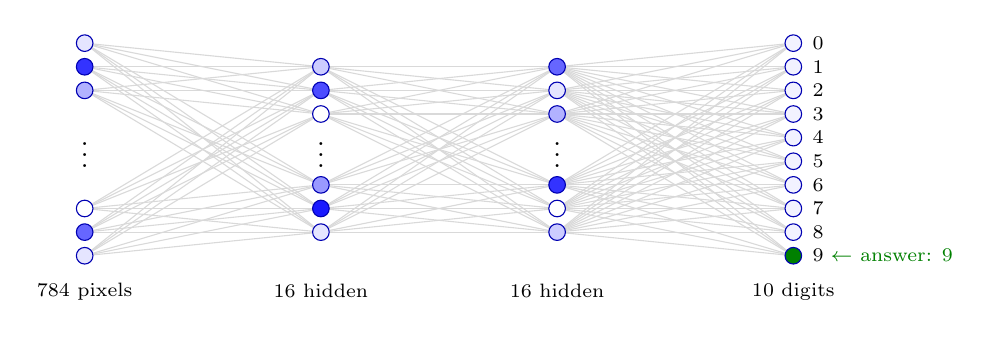
\begin{tikzpicture}[x=1cm, y=0.3cm,
    nrn/.style={circle, draw=blue!70!black, minimum size=6pt, inner sep=0pt}]
\foreach \a in {4.5,3.5,2.5,-2.5,-3.5,-4.5}
  \foreach \b in {3.5,2.5,1.5,-1.5,-2.5,-3.5}
    \draw[gray!30] (0,\a) -- (3,\b);
\foreach \a in {3.5,2.5,1.5,-1.5,-2.5,-3.5}
  \foreach \b in {3.5,2.5,1.5,-1.5,-2.5,-3.5}
    \draw[gray!30] (3,\a) -- (6,\b);
\foreach \a in {3.5,2.5,1.5,-1.5,-2.5,-3.5}
  \foreach \b in {4.5,3.5,...,-4.5}
    \draw[gray!30] (6,\a) -- (9,\b);
\foreach \y/\s in {4.5/10, 3.5/80, 2.5/30, -2.5/0, -3.5/60, -4.5/10}
  \node[nrn, fill=blue!\s] at (0,\y) {};
\node at (0,0.1) {$\vdots$};
\foreach \y/\s in {3.5/20, 2.5/70, 1.5/0, -1.5/40, -2.5/90, -3.5/10}
  \node[nrn, fill=blue!\s] at (3,\y) {};
\node at (3,0.1) {$\vdots$};
\foreach \y/\s in {3.5/60, 2.5/10, 1.5/30, -1.5/80, -2.5/0, -3.5/20}
  \node[nrn, fill=blue!\s] at (6,\y) {};
\node at (6,0.1) {$\vdots$};
\foreach \d [evaluate=\d as \y using 4.5-\d] in {0,...,8}
  \node[nrn, fill=blue!5] at (9,\y) {};
\node[nrn, fill=green!50!black] at (9,-4.5) {};
\foreach \d [evaluate=\d as \y using 4.5-\d] in {0,...,9}
  \node[font=\scriptsize, anchor=west] at (9.12,\y) {\d};
\node[font=\scriptsize, green!50!black, anchor=west] at (9.35,-4.5) {$\leftarrow$ answer: 9};
\node[font=\scriptsize] at (0,-6) {784 pixels};
\node[font=\scriptsize] at (3,-6) {16 hidden};
\node[font=\scriptsize] at (6,-6) {16 hidden};
\node[font=\scriptsize] at (9,-6) {10 digits};
\end{tikzpicture}
\par}
\end{keeptogether}

\begin{keeptogether}
\textbf{Why layers?} We recognize a 9 as a loop on top plus a line on the right. The hope is that each layer builds bigger parts from the last one's (not guaranteed after training). Same idea elsewhere: speech is sounds $\to$ syllables $\to$ words.

{\centering
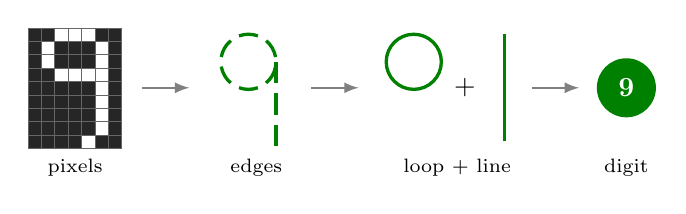
\begin{tikzpicture}[x=1cm, y=1cm]
\begin{scope}[x=0.17cm, y=0.17cm]
\fill[black!85] (0,0) rectangle (7,9);
\foreach \c/\r in {2/8,3/8,4/8, 1/7,5/7, 1/6,5/6, 2/5,3/5,4/5,5/5, 5/4, 5/3, 5/2, 5/1, 4/0}
  \fill[white] (\c,\r) rectangle ++(1,1);
\draw[black!60, very thin, step=1] (0,0) grid (7,9);
\end{scope}
\node[font=\scriptsize] at (0.6,-0.25) {pixels};
\draw[-latex, thick, gray] (1.45,0.77) -- (2.05,0.77);
\begin{scope}[shift={(2.8,0)}]
\foreach \a in {0,60,...,300}
  \draw[very thick, green!50!black] ([shift={(0,1.1)}]\a+10:0.35) arc[start angle=\a+10, end angle=\a+50, radius=0.35];
\foreach \y in {1.1,0.7,0.3}
  \draw[very thick, green!50!black] (0.35,\y) -- (0.35,\y-0.27);
\end{scope}
\node[font=\scriptsize] at (2.9,-0.25) {edges};
\draw[-latex, thick, gray] (3.6,0.77) -- (4.2,0.77);
\begin{scope}[shift={(4.9,0)}]
\draw[very thick, green!50!black] (0,1.1) circle (0.35);
\node at (0.65,0.77) {$+$};
\draw[very thick, green!50!black] (1.15,1.45) -- (1.15,0.1);
\end{scope}
\node[font=\scriptsize] at (5.45,-0.25) {loop + line};
\draw[-latex, thick, gray] (6.4,0.77) -- (7.0,0.77);
\node[circle, fill=green!50!black, text=white, minimum size=0.75cm, font=\bfseries] at (7.6,0.77) {9};
\node[font=\scriptsize] at (7.6,-0.25) {digit};
\end{tikzpicture}
\par}
\end{keeptogether}

\subsection*{One Neuron: Weights, Sigmoid, Bias}
How does one neuron's activation come from the previous layer?

\begin{keeptogether}
\textbf{Example: detecting an edge.} Say we want one neuron to light up only when the image has a short horizontal edge in one specific spot (like the middle bar of a 3). Give the neuron one \textbf{weight} per pixel, and draw the weights as a grid in the same layout as the image:
\begin{itemize}
  \item \textbf{Green} ($w = +1$): the 5 pixels where the edge should be. A bright pixel here \textbf{adds} to the sum.
  \item \textbf{Red} ($w = -1$): the 10 pixels just above and below. A bright pixel here \textbf{subtracts} from the sum.
  \item \textbf{Blank} ($w = 0$): every other pixel. Ignored.
\end{itemize}

{\centering
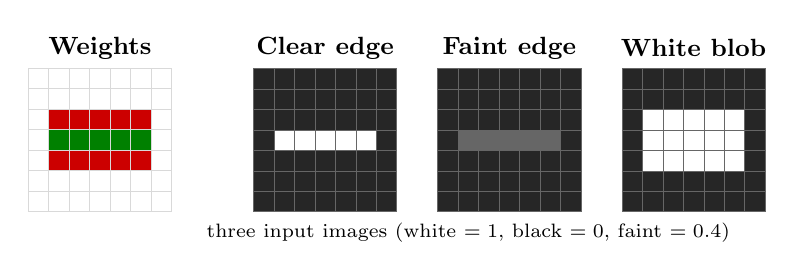
\begin{tikzpicture}[x=0.26cm, y=0.26cm]
% weights
\begin{scope}
\foreach \c in {1,...,5} \fill[green!50!black] (\c,3) rectangle ++(1,1);
\foreach \c in {1,...,5} \fill[red!80!black] (\c,2) rectangle ++(1,1);
\foreach \c in {1,...,5} \fill[red!80!black] (\c,4) rectangle ++(1,1);
\draw[gray!30, step=1] (0,0) grid (7,7);
\node[font=\small\bfseries] at (3.5,8) {Weights};
\end{scope}
% clear line
\begin{scope}[shift={(11,0)}]
\fill[black!85] (0,0) rectangle (7,7);
\foreach \c in {1,...,5} \fill[white] (\c,3) rectangle ++(1,1);
\draw[black!60, very thin, step=1] (0,0) grid (7,7);
\node[font=\small\bfseries] at (3.5,8) {Clear edge};
\end{scope}
% faint line
\begin{scope}[shift={(20,0)}]
\fill[black!85] (0,0) rectangle (7,7);
\foreach \c in {1,...,5} \fill[white!40!black] (\c,3) rectangle ++(1,1);
\draw[black!60, very thin, step=1] (0,0) grid (7,7);
\node[font=\small\bfseries] at (3.5,8) {Faint edge};
\end{scope}
% white blob
\begin{scope}[shift={(29,0)}]
\fill[black!85] (0,0) rectangle (7,7);
\foreach \r in {2,3,4} \foreach \c in {1,...,5} \fill[white] (\c,\r) rectangle ++(1,1);
\draw[black!60, very thin, step=1] (0,0) grid (7,7);
\node[font=\small\bfseries] at (3.5,8) {White blob};
\end{scope}
\node[font=\scriptsize] at (21.5,-1) {three input images (white $= 1$, black $= 0$, faint $= 0.4$)};
\end{tikzpicture}
\par}
\end{keeptogether}

\begin{keeptogether}
\textbf{Step 1: Weighted sum.} Multiply each input by its weight and add up:
\[
w_1 x_1 + w_2 x_2 + w_3 x_3 + \cdots + w_D x_D
\]
In the example, the $x_j$'s are the pixels and only the 15 green and red pixels count:
\[
\text{Clear: } 5(1) - 10(0) = 5,
\qquad
\text{Faint: } 5(0.4) - 10(0) = 2,
\qquad
\text{Blob: } 5(1) - 10(1) = -5
\]
\end{keeptogether}

\begin{keeptogether}
\textbf{Step 2: Squish with the sigmoid.} The sum can be any number, but an activation should be between 0 and 1. Wrap it in the \textbf{sigmoid} $\sigma(z) = \frac{1}{1 + e^{-z}}$ (very negative $\to$ near 0, very positive $\to$ near 1):
\[
\sigma\big(w_1 x_1 + w_2 x_2 + w_3 x_3 + \cdots + w_D x_D\big)
\]
\[
\text{Clear: } \sigma(5) = 0.99,
\qquad
\text{Faint: } \sigma(2) = 0.88,
\qquad
\text{Blob: } \sigma(-5) = 0.01
\]
Problem: the faint edge (0.88) lights up almost as much as the clear one.
\end{keeptogether}

\begin{keeptogether}
\textbf{Step 3: Add a bias.} We only want the neuron on when the sum is clearly big (above about 3). So add a \textbf{bias} $b$ before squishing:
\[
\sigma\big(w_1 x_1 + w_2 x_2 + w_3 x_3 + \cdots + w_D x_D + b\big)
\]
With $b = -3$:
\[
\text{Clear: } \sigma(5 - 3) = 0.88,
\qquad
\text{Faint: } \sigma(2 - 3) = 0.27,
\qquad
\text{Blob: } \sigma(-5 - 3) = 0.00
\]

{\centering
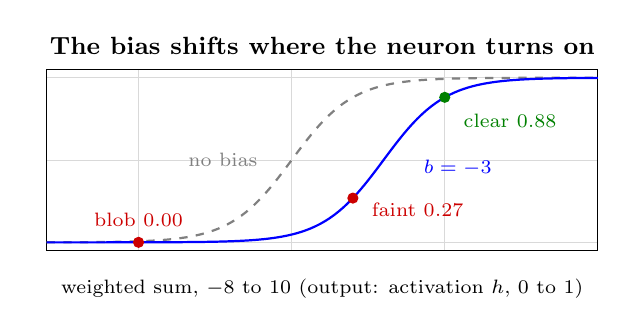
\begin{tikzpicture}
\begin{axis}[scale only axis, width=7cm, height=2.3cm,
    xmin=-8, xmax=10, ymin=-0.05, ymax=1.05, enlargelimits=false,
    grid=major, grid style={gray!30}, major tick length=0pt,
    xticklabels={}, yticklabels={},
    title={\small\textbf{The bias shifts where the neuron turns on}}, title style={yshift=-4pt},
    xlabel={\scriptsize weighted sum, $-8$ to $10$ (output: activation $h$, 0 to 1)}, label style={font=\scriptsize}]
\addplot[thick, gray, dashed, domain=-8:10, samples=120] {1/(1+exp(-x))};
\addplot[thick, blue, domain=-8:10, samples=120] {1/(1+exp(-(x-3)))};
\addplot[only marks, mark=*, green!50!black, mark size=1.8pt] coordinates {(5,0.881)};
\addplot[only marks, mark=*, red!80!black, mark size=1.8pt] coordinates {(2,0.269) (-5,0.0003)};
\node[font=\scriptsize, green!50!black, anchor=north west] at (axis cs:5.3,0.84) {clear $0.88$};
\node[font=\scriptsize, red!80!black, anchor=west] at (axis cs:2.3,0.2) {faint $0.27$};
\node[font=\scriptsize, red!80!black, anchor=south] at (axis cs:-5,0.04) {blob $0.00$};
\node[font=\scriptsize, gray, anchor=east] at (axis cs:-0.8,0.5) {no bias};
\node[font=\scriptsize, blue, anchor=west] at (axis cs:4,0.45) {$b = -3$};
\end{axis}
\end{tikzpicture}
\par}
\end{keeptogether}

\begin{keeptogether}
\textbf{Putting it together.} That's all a neuron does. Every neuron works this way with its own weights and bias, and its inputs $x_1, \dots, x_D$ are the activations of every neuron in the previous layer:

{\centering
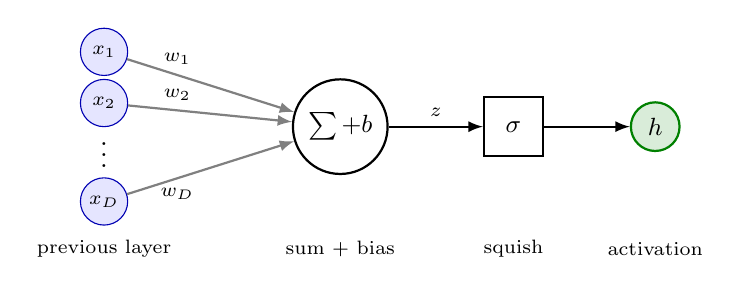
\begin{tikzpicture}[x=1cm, y=1cm, >=latex,
    inp/.style={circle, draw=blue!70!black, fill=blue!10, minimum size=0.6cm, inner sep=0pt, font=\scriptsize}]
\node[inp] (x1) at (0,0.95) {$x_1$};
\node[inp] (x2) at (0,0.3) {$x_2$};
\node at (0,-0.25) {$\vdots$};
\node[inp] (xD) at (0,-0.95) {$x_D$};
\node[circle, draw, thick, minimum size=1cm, font=\small] (sum) at (3,0) {$\sum + b$};
\draw[->, thick, gray] (x1) -- node[pos=0.3, above, font=\scriptsize, black] {$w_1$} (sum);
\draw[->, thick, gray] (x2) -- node[pos=0.3, above, font=\scriptsize, black] {$w_2$} (sum);
\draw[->, thick, gray] (xD) -- node[pos=0.3, below, font=\scriptsize, black] {$w_D$} (sum);
\node[draw, thick, minimum size=0.75cm, font=\small] (sig) at (5.2,0) {$\sigma$};
\draw[->, thick] (sum) -- node[above, font=\scriptsize] {$z$} (sig);
\node[circle, draw=green!50!black, fill=green!50!black!15, thick, minimum size=0.6cm, font=\small] (h) at (7,0) {$h$};
\draw[->, thick] (sig) -- (h);
\node[font=\scriptsize] at (0,-1.55) {previous layer};
\node[font=\scriptsize] at (3,-1.55) {sum + bias};
\node[font=\scriptsize] at (5.2,-1.55) {squish};
\node[font=\scriptsize] at (7,-1.55) {activation};
\end{tikzpicture}
\par}
Written compactly:
\[
h = \sigma\Big(\underbrace{\textstyle\sum_{j=1}^{D} w_j x_j}_{\text{weighted sum}} + \underbrace{b}_{\text{bias}}\Big) = \sigma(\mathbf{w}^\top \mathbf{x} + b)
\]
The \textbf{weights} decide which pattern the neuron looks for (the green/red grid); the \textbf{bias} decides how strong the pattern must be before the neuron lights up ($b = -3$).
\end{keeptogether}

\subsection*{A Layer as a Matrix Product}
\begin{keeptogether}
A layer is $M$ neurons, and \textbf{every neuron connects to every neuron in the previous layer} $x_1, \dots, x_D$. Neuron $i$'s weights (green) become \textbf{row $i$} of $\mathbf{W}$:

{\centering
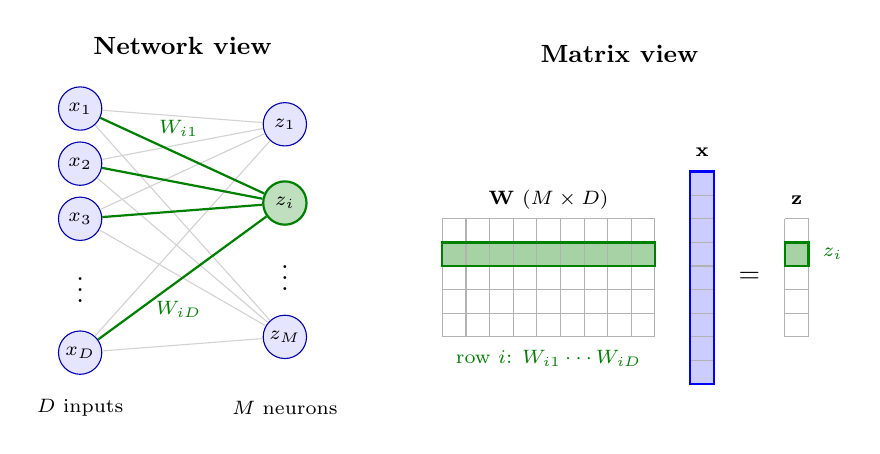
\begin{tikzpicture}[>=latex,
    nrn/.style={circle, draw=blue!70!black, fill=blue!10, minimum size=0.55cm, inner sep=0pt, font=\scriptsize}]
% ---- network view ----
\foreach \n/\y in {1/1.8, 2/1.1, 3/0.4, D/-1.3}
  \node[nrn] (x\n) at (0,\y) {$x_{\n}$};
\node at (0,-0.4) {$\vdots$};
\node[nrn] (z1) at (2.6,1.6) {$z_1$};
\node[nrn, draw=green!50!black, fill=green!50!black!25, thick] (zi) at (2.6,0.6) {$z_i$};
\node at (2.6,-0.25) {$\vdots$};
\node[nrn] (zM) at (2.6,-1.1) {$z_M$};
\foreach \n in {1,2,3,D} \foreach \m in {1,M}
  \draw[gray!35] (x\n) -- (z\m);
\foreach \n in {1,2,3,D}
  \draw[green!50!black, thick] (x\n) -- (zi);
\node[font=\scriptsize, green!50!black] at (1.25,1.55) {$W_{i1}$};
\node[font=\scriptsize, green!50!black] at (1.25,-0.75) {$W_{iD}$};
\node[font=\scriptsize] at (0,-2) {$D$ inputs};
\node[font=\scriptsize] at (2.6,-2) {$M$ neurons};
\node[font=\small\bfseries] at (1.3,2.6) {Network view};
% ---- matrix view ----
\begin{scope}[shift={(4.6,-1.1)}, x=0.3cm, y=0.3cm]
\fill[green!50!black!35] (0,3) rectangle (9,4);
\draw[gray!60, step=1] (0,0) grid (9,5);
\draw[green!50!black, thick] (0,3) rectangle (9,4);
\node[font=\scriptsize] at (4.5,5.8) {$\mathbf{W}$ ($M \times D$)};
\node[font=\scriptsize, green!50!black] at (4.5,-0.9) {row $i$: $W_{i1} \cdots W_{iD}$};
\fill[blue!20] (10.5,-2) rectangle (11.5,7);
\draw[gray!60, step=1, xshift=0.15cm] (10,-2) grid (11,7);
\draw[blue, thick] (10.5,-2) rectangle (11.5,7);
\node[font=\scriptsize] at (11,7.8) {$\mathbf{x}$};
\node at (13,2.5) {$=$};
\fill[green!50!black!35] (14.5,3) rectangle ++(1,1);
\draw[gray!60, step=1, xshift=0.15cm] (14,0) grid (15,5);
\draw[green!50!black, thick] (14.5,3) rectangle ++(1,1);
\node[font=\scriptsize] at (15,5.8) {$\mathbf{z}$};
\node[font=\scriptsize, green!50!black, anchor=west] at (15.7,3.5) {$z_i$};
\node[font=\small\bfseries] at (7.5,12) {Matrix view};
\end{scope}
\end{tikzpicture}
\par}
\[
z_i = \sum_{j=1}^{D} W_{ij}\, x_j + b_i \qquad (W_{ij} = \text{weight into neuron } i \text{ from input } j)
\]
\end{keeptogether}

\begin{keeptogether}
\textbf{The whole layer at once.} A layer with $D$ inputs and $M$ units (digit net, first hidden layer: $D = 784$, $M = 16$):
\[
\underbrace{\begin{bmatrix}
W_{11} & \cdots & W_{1D} \\
\vdots & \ddots & \vdots \\
W_{M1} & \cdots & W_{MD}
\end{bmatrix}}_{\mathbf{W}\ (M \times D)}
\underbrace{\begin{bmatrix} x_1 \\ \vdots \\ x_D \end{bmatrix}}_{\mathbf{x}}
+
\underbrace{\begin{bmatrix} b_1 \\ \vdots \\ b_M \end{bmatrix}}_{\mathbf{b}}
=
\underbrace{\begin{bmatrix} z_1 \\ \vdots \\ z_M \end{bmatrix}}_{\mathbf{z}},
\qquad
\mathbf{h} = \sigma(\mathbf{z}) \text{ (each entry)}
\]
\end{keeptogether}

\begin{keeptogether}
\textbf{Small example} (2 neurons, 3 inputs):
\[
\begin{bmatrix} 1 & 0 & -1 \\ 0 & 2 & 0 \end{bmatrix}
\begin{bmatrix} 0.9 \\ 0.5 \\ 0.1 \end{bmatrix}
+
\begin{bmatrix} -0.5 \\ 0 \end{bmatrix}
=
\begin{bmatrix} 0.9 - 0.1 - 0.5 \\ 2(0.5) \end{bmatrix}
=
\begin{bmatrix} 0.3 \\ 1.0 \end{bmatrix}
\ \xrightarrow{\ \sigma\ }\
\begin{bmatrix} 0.57 \\ 0.73 \end{bmatrix}
\]
\end{keeptogether}

\begin{keeptogether}
\textbf{Every layer} works the same way, one matrix product per layer, starting from $\mathbf{h}^{(0)} = \mathbf{x}$.
\[
\mathbf{z}^{(l)} = \mathbf{W}^{(l)} \mathbf{h}^{(l-1)} + \mathbf{b}^{(l)},
\qquad
\mathbf{h}^{(l)} = \sigma\big(\mathbf{z}^{(l)}\big)
\]
\end{keeptogether}
Each layer has $D_{\text{out}}(D_{\text{in}} + 1)$ parameters (weights + biases), so the digit net has:
\[
\underbrace{16(784 + 1)}_{\text{input} \to \text{hidden 1}}
+ \underbrace{16(16 + 1)}_{\text{hidden 1} \to \text{hidden 2}}
+ \underbrace{10(16 + 1)}_{\text{hidden 2} \to \text{output}}
= 13{,}002 \text{ parameters}
\]

\subsection*{The Network Is Just a Function}
\begin{keeptogether}
Each neuron takes in the previous layer's outputs and spits out one number. Chain the layers and the whole network is one (very complicated) function: 784 numbers in, 10 numbers out, 13{,}002 parameters.
\[
\hat{\mathbf{y}} = \sigma\Big(\mathbf{W}^{(3)}\, \sigma\big(\mathbf{W}^{(2)}\, \underbrace{\sigma(\mathbf{W}^{(1)}\mathbf{x} + \mathbf{b}^{(1)})}_{\text{hidden layer 1}} + \mathbf{b}^{(2)}\big) + \mathbf{b}^{(3)}\Big)
\]
\end{keeptogether}

